\documentclass[a4paper]{jpconf}
%\bibliographystyle{iopart-num}
%\usepackage{citesort}
\usepackage{graphicx}

\begin{document}
\title{A Geant4 physics list for spallation and related nuclear physics applications 
based on INCL and ABLA models}

\author{A Heikkinen$^1$, A Boudard$^2$, P Kaitaniemi$^{1,2}$ and G Folger$^3$}

%\author{P J Smith$^1$, T M Collins$^2$, 
%R J Jones$^{3,}$\footnote[4]{Present address:
%Department of Physics, University of Bristol, Tyndalls Park Road, 
%Bristol BS8 1TS, UK.} and Janet Williams$^3$}

\address{$^1$ Helsinki Institute of Physics, P.O. Box 64, FIN-00014 University of Helsinki, Finland}
\address{$^2$ CEN-Saclay, CEA-IRFU/SPhN, 91 191 Gif sur Yvette, France}
\address{$^3$ European Organization for Nuclear Research (CERN), Switzerland}

\ead{aatos.heikkinen@cern.ch}

\begin{abstract}
We present a new Geant4 physics list prepared for nuclear physics applications
in the domain dominated by spallation.
We discuss new Geant4 physics of the C++ translation of original Fortran 
INCL intra-nuclear cascade and ABLA fission/de-excitation codes.
that are used in the physic list.
The INCL model is well established for targets heavier than Aluminium
and projectile energies from $\sim$ 150 MeV up to 2.5 GeV $\sim$ 3 GeV.
Validity of the Geant4 physics list is demonstrated from the perspective of accelerator driven systems
and EURISOL project, especially with the neutron double differential cross sections and residual
nuclei production.
Foreseen improvements of the physics models for the treatment of light targets (Carbon - Oxygen)
and light ion beams (up to Carbon) are discussed.
An example application utilizing the physics list is introduced.
\end{abstract}

\section{Introduction} \label{sec:intro}
In this paper we are interested on issues relevant Geant4 simulation of nuclear physics applications,
neutron production and modeling of spallation reactions.  


%\subsection{Accelerator Driven Systems}
%ADS
% Material: http://users.ictp.it/~pub_off/lectures/lns012/Kadi_002.pdf
One of our motivation is to  develop Geant4 tools
 for simulation of Accelerator Drive System (ADS)
The goal of accelerator driven sub-critical reactor 
development is to provide safer and more effective
methods of nuclear power production. 
The main components of an ADS system are: accelerator, spallation
target and sub-critical core.


The most important benefits of
this new type of reactor include improved safety. In case of an
emergency the accelerator can be shut down which in turn shuts down
the reactor. Another important safety benefit is that the system
transmutes nuclear waste to less harmful isotopes.


To this aim we present a new Geant4 physics list, 
based on INCL \cite{incl} intra-nuclear cascade model and ABLA model in Geant4 9.2~\cite{g4}. 


%The INCL model is well established for targets heavier than Aluminium
%and projectile energies from $\sim$ 150 MeV up to 2.5 GeV $\sim$ 3 GeV . 


This paper is organized as follows.
Section~\ref{sec:list} briefly summarise the concept of physics list.
Geant4 9.2 models intra-nuclear cascade INCL or Liege cascade, and ABLA evaporation-fission model
applied in this work are introduced in Section~\ref{sec:models},
Section~\ref{sec:newlist} documents the details of physics list implementation, 
%Secctio~\ref{sec:example} describes an example application utilizing the new physics list
%for the use case of spallation reaction study.
Physics performance is demonstrated particularly for 
neutron  cross sections in Section~\ref{sec:performance} and
Section~\ref{sec:carbon} concludes with outline of future models developments.


\section{Geant4 physics lists}\label{sec:list}

A unique feature of Geant4 is to  
decouple physics models, cross sections, and processes
using abstract interfaces, and manage the usage of different options with so-called the physics lists:
\begin{itemize}
\item Physics lists allow users to find good balance between various goals (e.g. CPU
time requirements vs. accuracy of results).
\item Also, the Geant4 physics system can be easily extended.
\end{itemize}

An unique feature of Geant4 is physics list concept providing transparent access 
to various physics models. 
Often an optional models are available with specific strengths and limitations, 
so physics lists concept is used to
provide optimal set of functionality for specific use case.

\section{INCL and ABLA models in Geant4} \label{sec:models}

INCL and ABLA models are casted into independent FORTRAN based Monte Carlo codes 
INCL4.2 and ABLA V3 \cite{heikkinen07mProceedings}.
Recently these implementations have been translated into C++ and codes distributed
as part of Geant4 toolkit \cite{heikkinen03aPaper}. 
First beta release of INCL 4.2 and ABLA v3 was in Geant4  9.1 (December 2007).

Currently new versions of INCL and ABLA versions in Geant4 are pure
FORTRAN to C++ translations. Our goal is to completely redesign the
INCL cascade code using modern OO techniques.

\section{A new Geant4 physics list {\tt QGSP\_\-INCL\_ABLA}}\label{sec:newlist}

We have implemented a new physics list called {\tt QGSP\_\-INCL\_ABLA} with
spallation physics in mind. 
It uses INCL/ABLA models for proton,
neutron and pion inelastic interactions in the energy range 0~-~3~GeV.

INCL/ABLA models can now be used via physics list {\tt
QGSP\_INCL\_ABLA}. The list is based on widely used {\tt QGSP\_BERT}
physics list. In the new list we use INCL/ABLA models instead of the
Bertini cascade.

The INCL/ABLA models are used for proton, neutron, pi+ and pi-
inelastic processes in the energy range 0 - 3 GeV. Above this
threshold QGSP model is used. Since this list is intended for
spallation and ADS applications we have not optimized the physics
performance for energies higher than 3 GeV. In order to extend the
list for high energy applications another model is probably needed
between QGSP and INCL/ABLA.

The class reference documentation of the INCL/ABLA models is produced
using Doxygen \cite{doxygen} documentation generator (see Fig.~\ref{fig:doxygen}). It allows us to
produce full documentation of the class structure complete with usage
instructions, class diagrams, detailed descriptions of all methods and
code listings.

\begin{figure}[h]
\begin{center}
%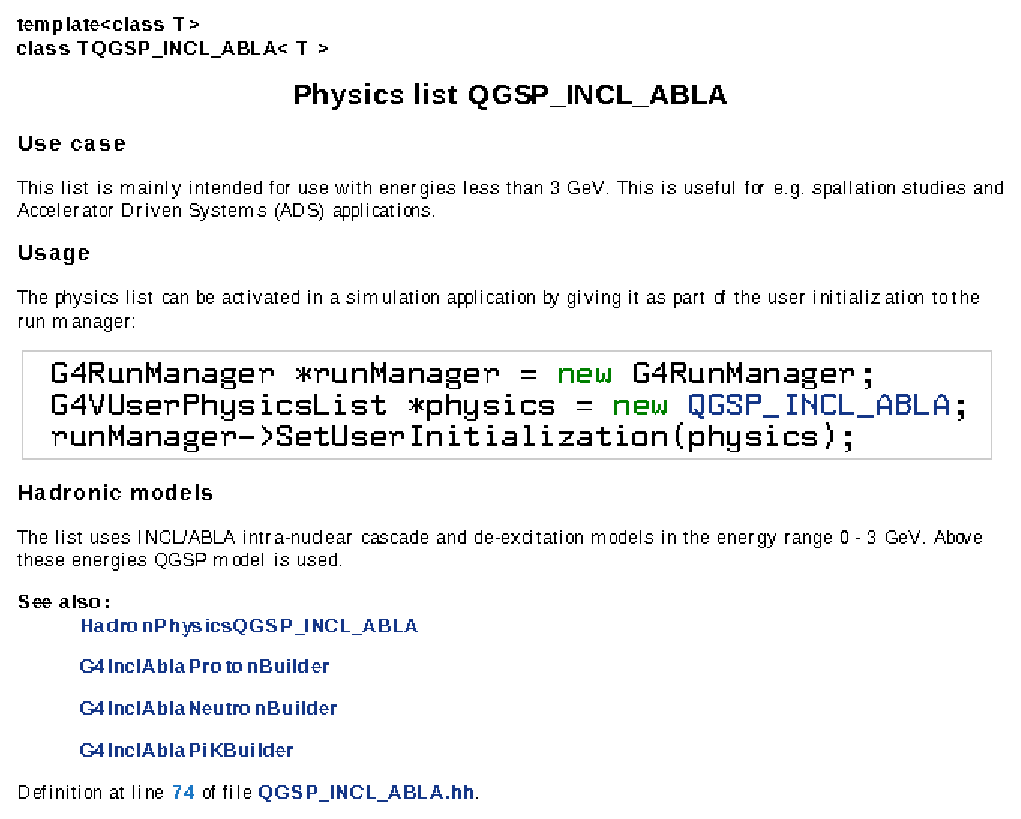
\includegraphics[width=21pc]{poster/images/inclAblaDoc.eps}\hspace{2pc}%
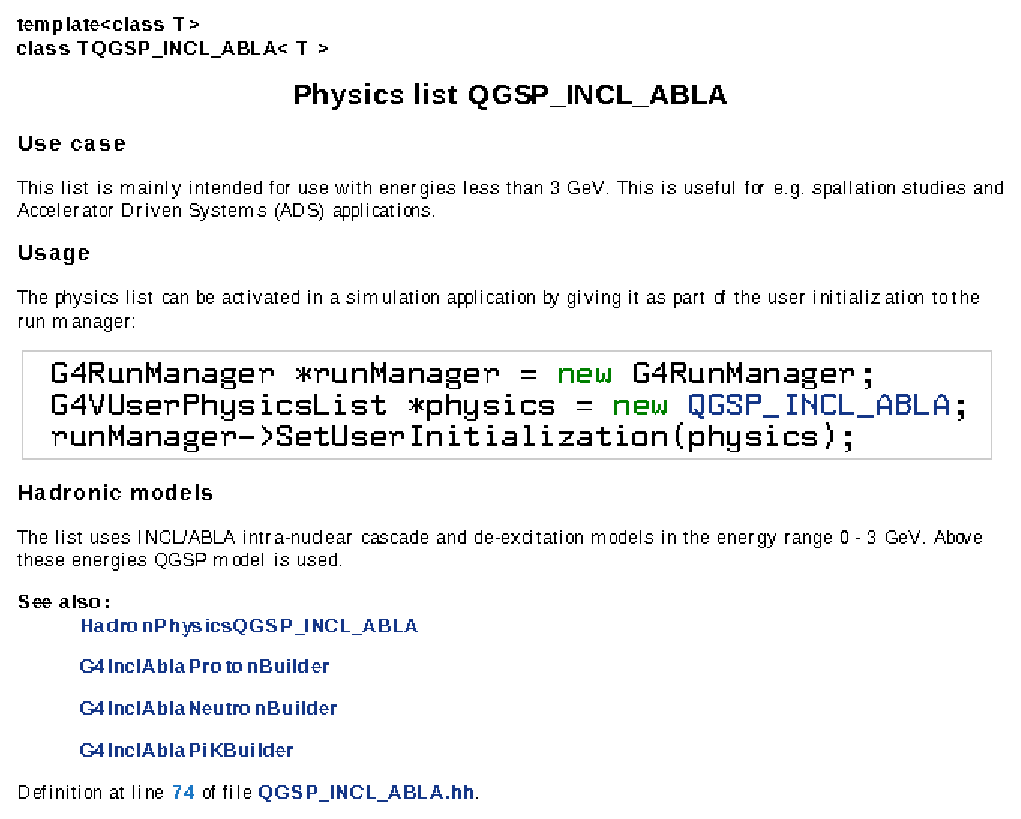
\includegraphics[scale=0.70]{poster/images/inclAblaDoc.eps}
%\begin{minipage}[b]{14pc}
\caption{\label{fig:doxygen}Doxygen documentation of Geant4 {\tt QGSP\_\-INCL\_ABLA} physics list is provided.}
%\end{minipage}
\end{center}
\end{figure}


\section{Physics performance}\label{sec:performance}
%\subsection{Fragment yield}
Fragment yield

\begin{figure}[h]
\begin{center}
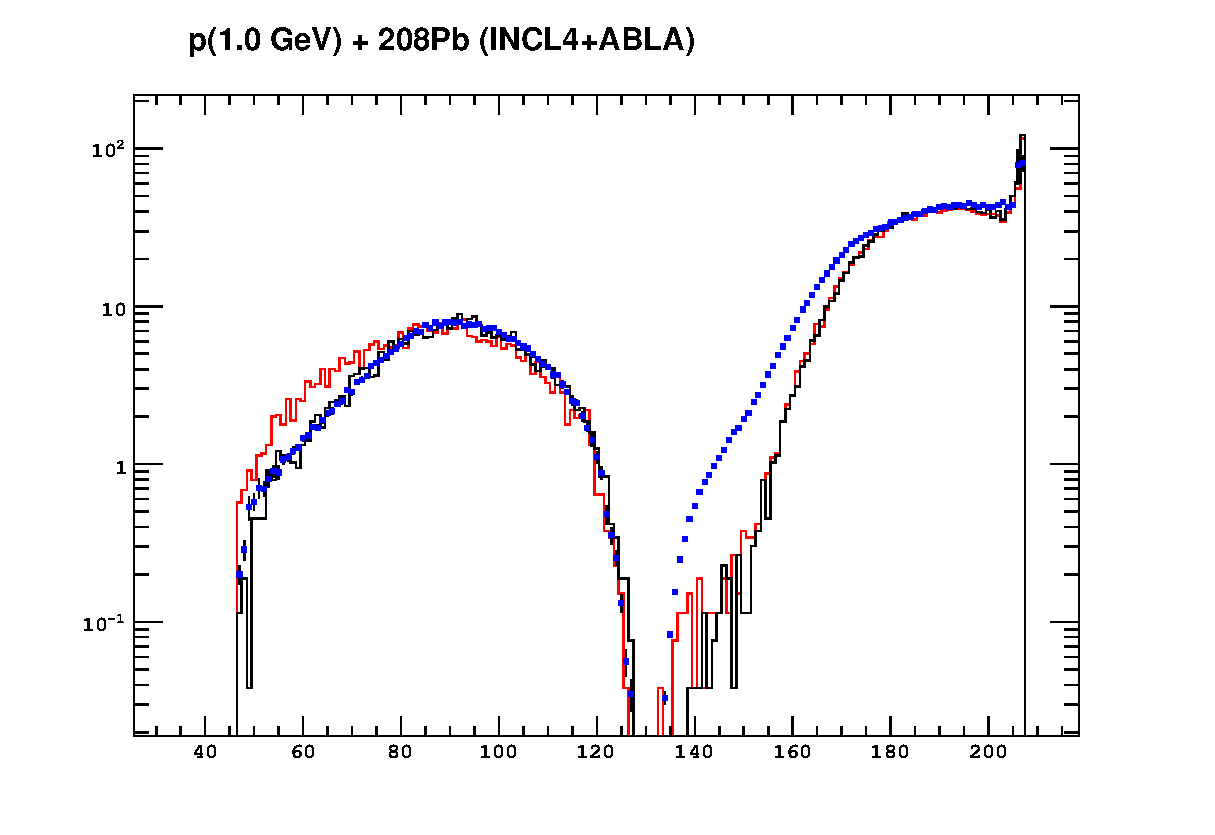
\includegraphics[scale=0.80]{poster/images/fragments.eps}

\caption{Fragment production of the INCL and ABLA \cite{abla, abla1, abla2} models. 
Black and red histograms are the results from the original FORTRAN version 
and new C++ implementation, respectively. Data is from Ref.~\cite{gsifragments}.}

\end{center}
\end{figure}


\begin{figure}[h]
\begin{center}
%Isotope production:
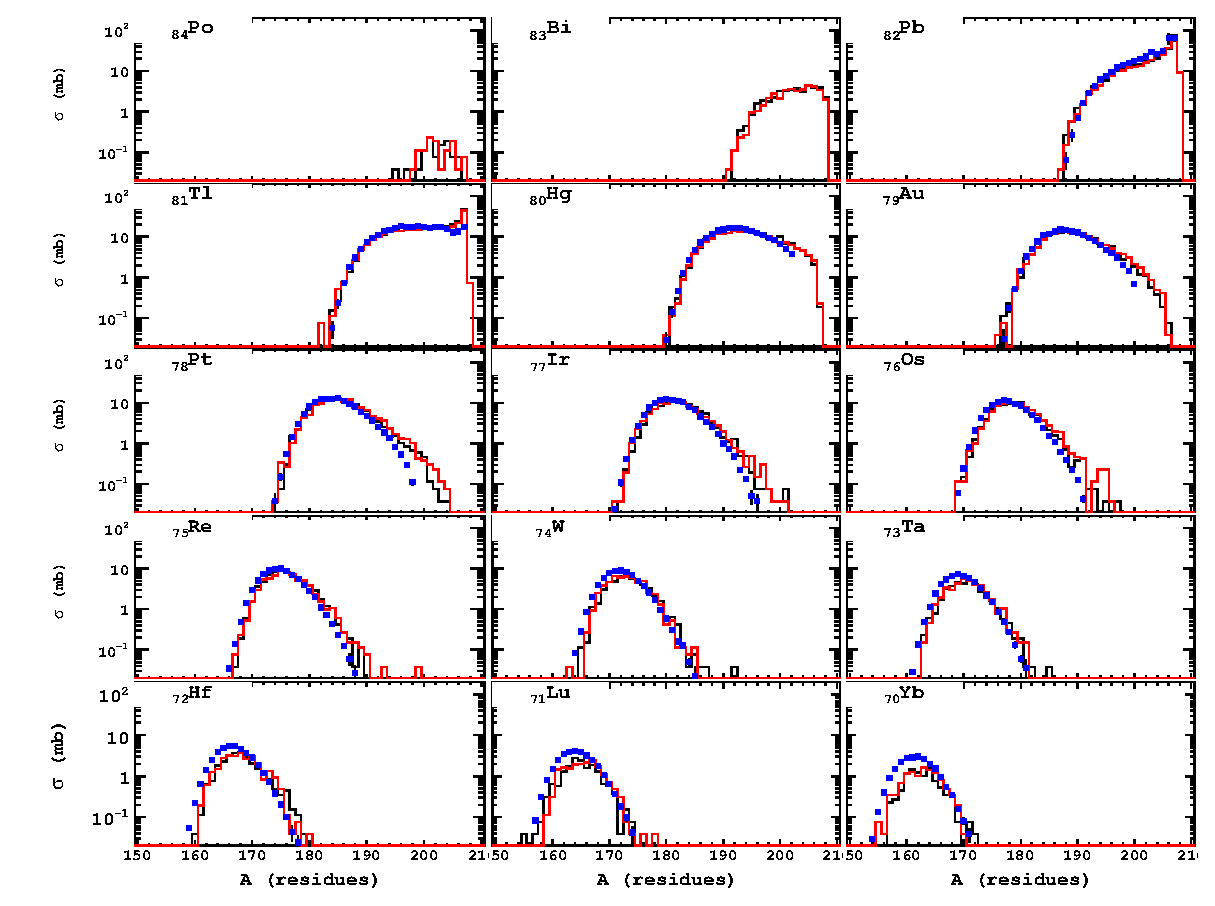
\includegraphics[scale=0.60]{poster/images/pPbIsotopes.eps}

\caption{Fragment production of the INCL and ABLA \cite{abla, abla1, abla2} models. 
Black and red histograms are the results from the original FORTRAN version 
and new C++ implementation, respectively. Data is from Ref. \cite{gsifragments}.}

\end{center}
\end{figure}


%\subsection{Neutron production}
Neutron production

\begin{figure}
\begin{center}
%\includegraphics[scale=0.5]{images/zirkonium.eps}
%\includegraphics[scale=0.5]{images/iron.eps}
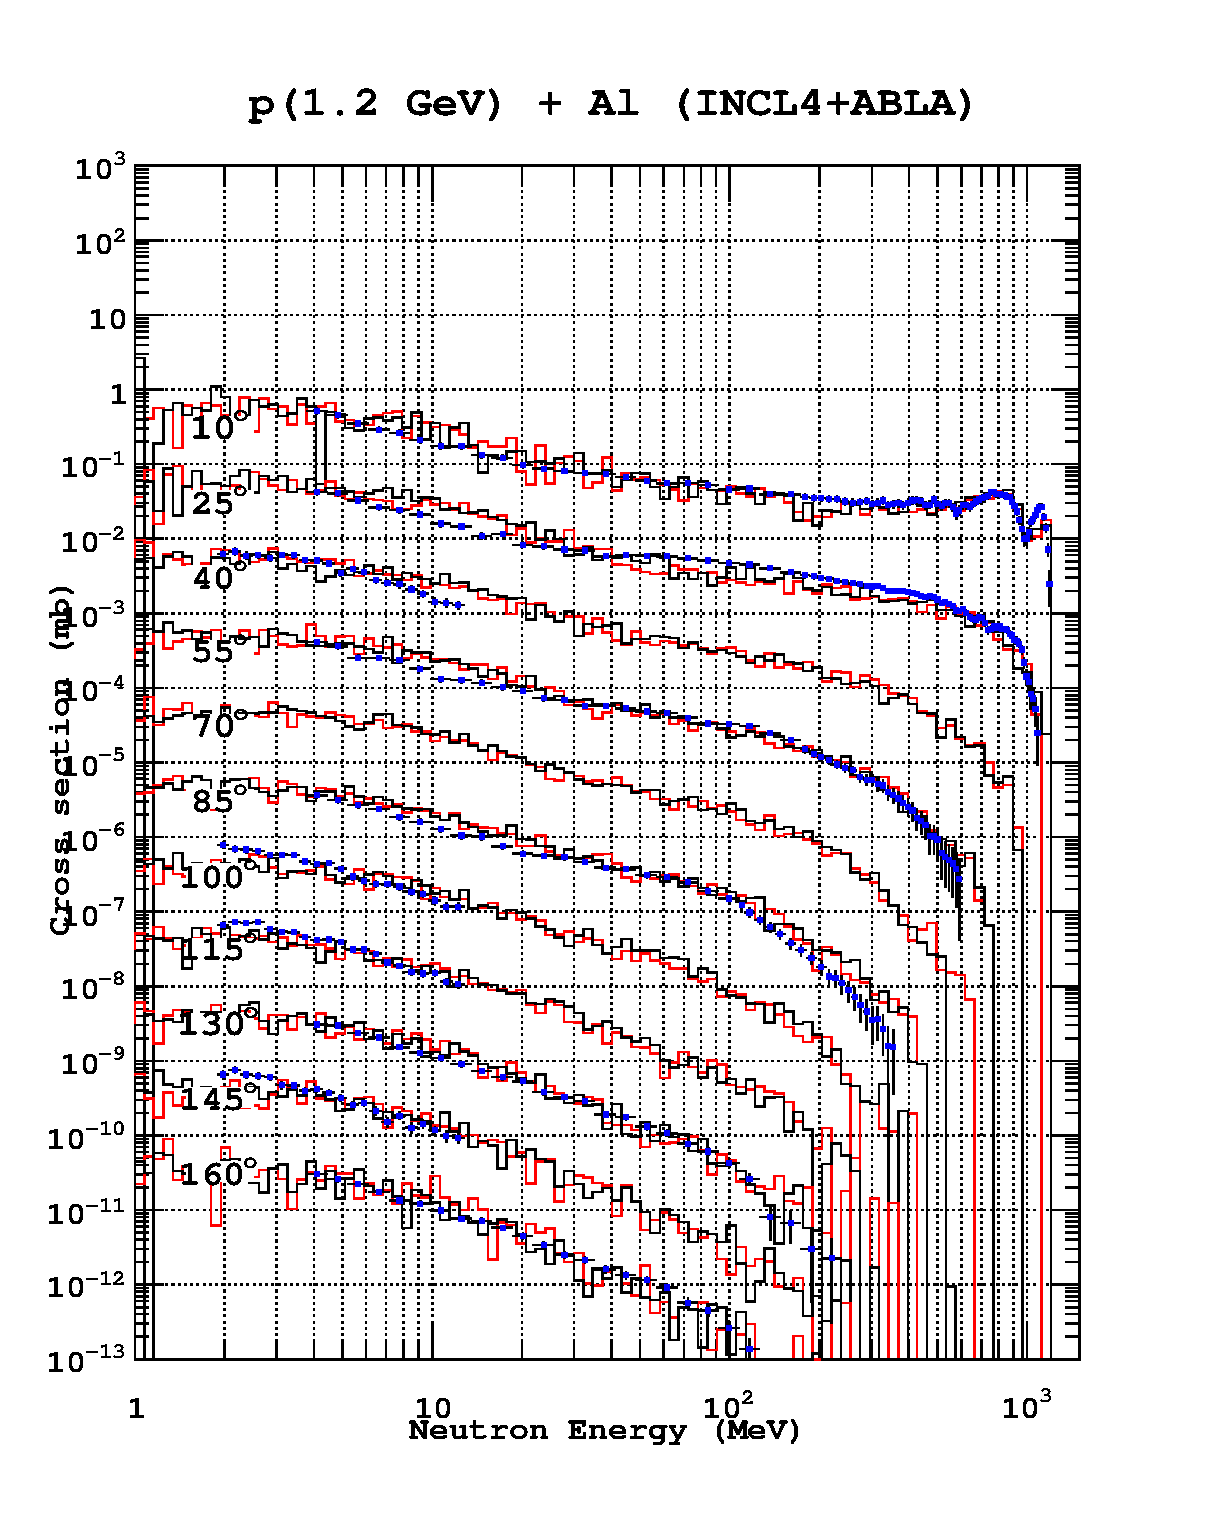
\includegraphics[scale=0.70]{poster/images/aluminum.eps}
\caption{Double-differential for neutron production cross section
    from Geant4 INCL and ABLA models in p(1.2 GeV) + Al $\rightarrow$ n + X reaction.
Black and red histograms are the
    results from the original FORTRAN version and new C++ implementation, respectively. 
Neutron evaporation from ABLA model is shown below E $\simeq$ 20 MeV.
Data is from Ref.~\cite{data}.}
\label{fig:neutronAl}
\end{center}
\end{figure}

\begin{figure}
\begin{center}
%\includegraphics[scale=0.5]{images/zirkonium.eps}
%\includegraphics[scale=0.5]{images/iron.eps}
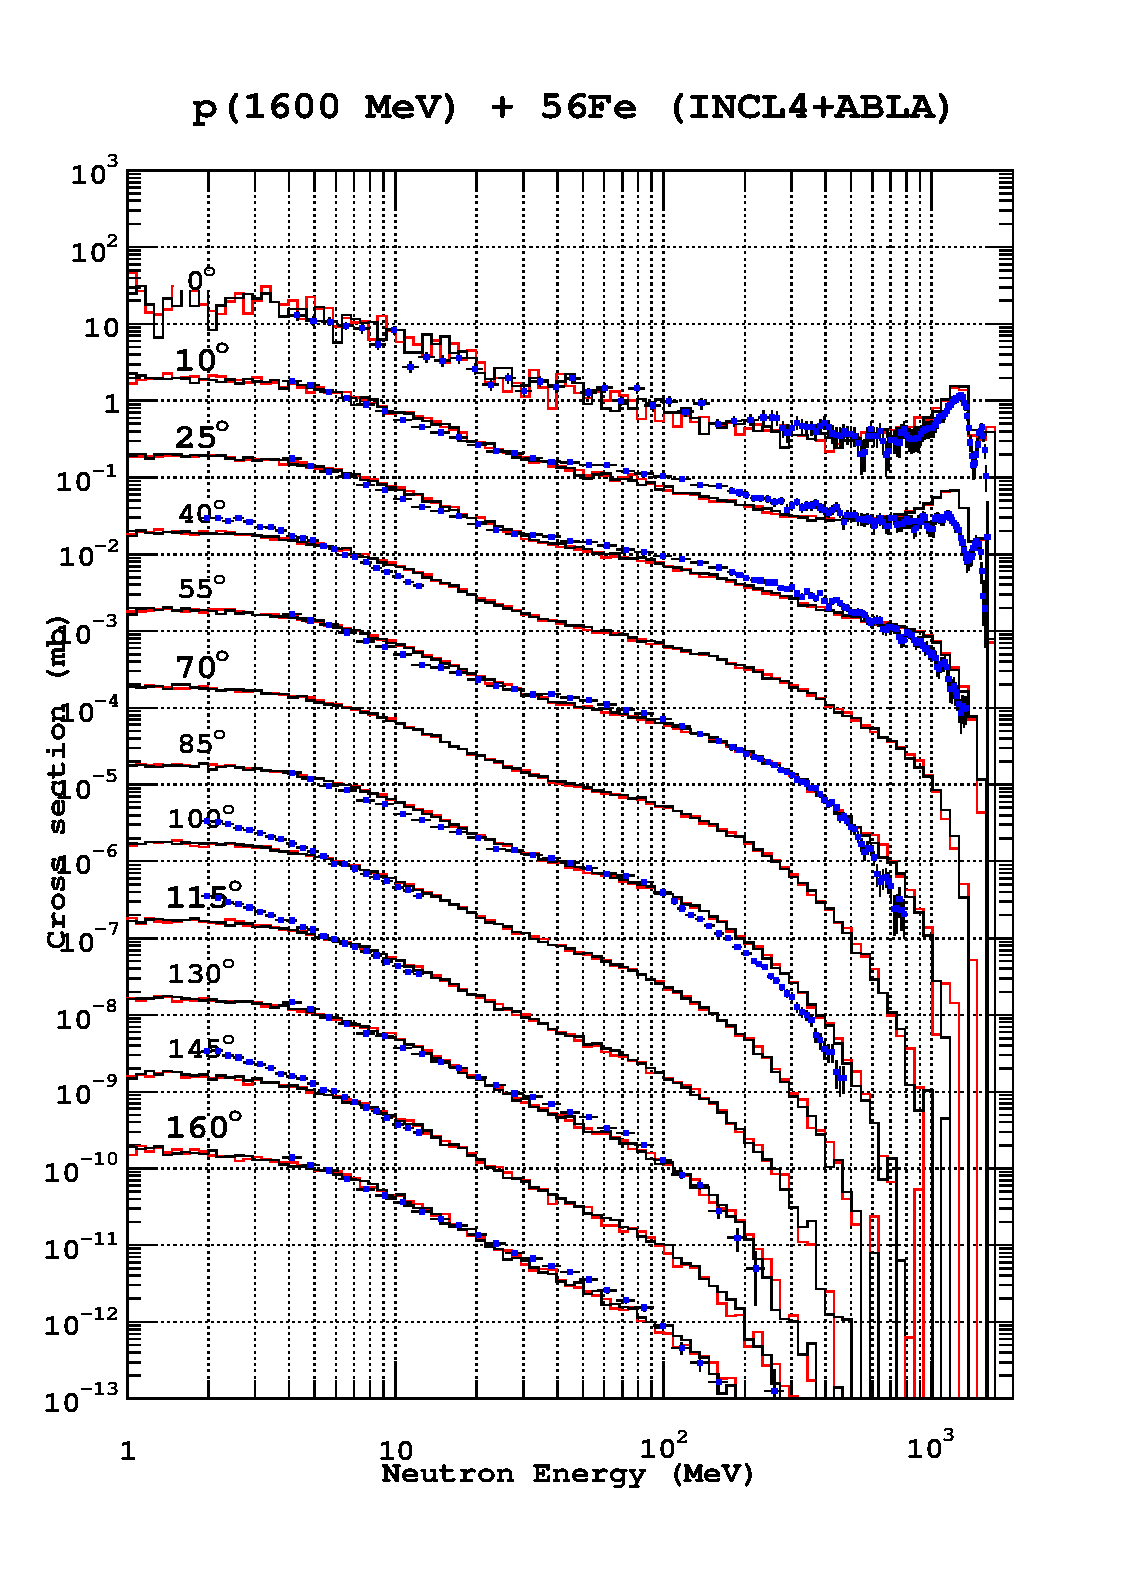
\includegraphics[scale=0.70]{images/proton1600MeVFe.eps}
\caption{Double-differential for neutron production cross section
    from Geant4 INCL and ABLA models in p(1.2 GeV) + Fe $\rightarrow$ n + X reaction.
Black and red histograms are the
    results from the original FORTRAN version and new C++ implementation, respectively. 
Neutron evaporation from ABLA model is shown below E $\simeq$ 20 MeV.
Data is from Ref.~\cite{data}.}
\label{fig:neutronAl}
\end{center}
\end{figure}


%\begin{figure}
%\begin{center}
%\includegraphics[scale=0.70]{poster/images/zirkonium.eps}
%\caption{Neutron production from p(1.2 GeV) + Zr $\rightarrow$ n + X.
%These results can be compared with a corresponding case with aluminium and iron targets show in Fig.~\ref{fig:neutronAl}
%and Fig.~\ref{fig:neutronFe}, respectively.}
%\end{center}
%\end{figure}

\begin{figure}
\begin{center}
\includegraphics[scale=0.70]{poster/images/iron.eps}
\caption{Neutron production from p(1.2 GeV) + Fe  $\rightarrow$ n + X. 
These results can be compared with a corresponding case with aluminium target in Fig.~\ref{fig:neutronAl}.}
\end{center}
\end{figure}



%\section{[commented in poster] p(1.2 GeV) + Pb $\rightarrow$ n + X}
%\begin{figure}
%\begin{center}
%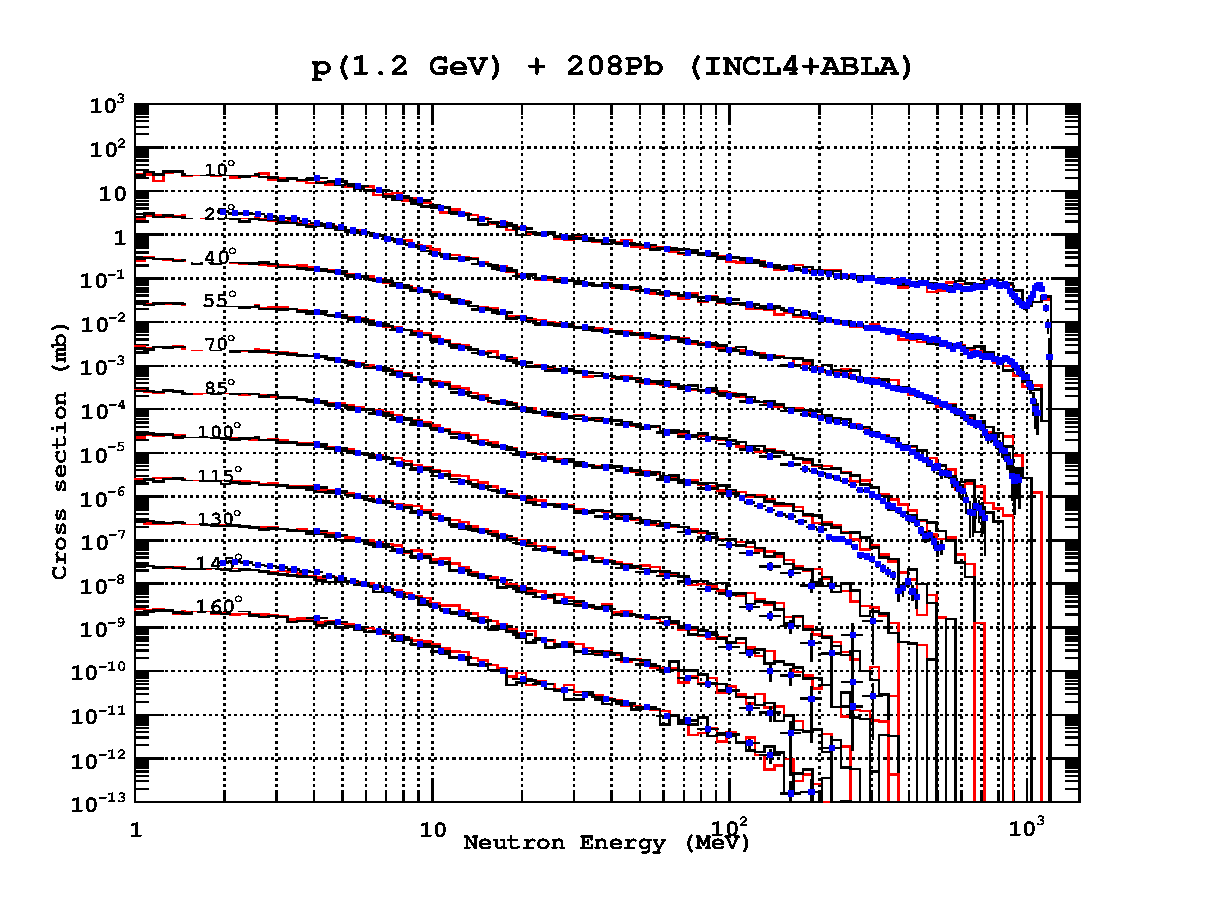
\includegraphics[scale=0.70]{poster/images/lead.eps}
%\end{center}
%\label{fig:pPbdd1200MeV}
%\caption{p(1.2 GeV) + Pb $\rightarrow$ n + X. Double-differential for neutron production cross section
%    from Geant4 INCL and ABLA models. Neutron evaporation from ABLA model is
%    shown below E $\simeq$ 20 MeV. Black and red histograms are the
%    results from the original FORTRAN version and new C++ implementation, respectively. 
%Blue data points are from Ref.~\cite{data}.}
%\end{figure}

%\subsection{Light targets}


%Light targets

We have introduced a cut to choose between ABLA and Fermi break-up for light targets.
So, INCL can now be used with the Geant4 Fermi break-up model.
Currently, INCL interface provides Fermi break-up \cite{g4incl} for
remnant nuclei lighter than A = 13 and ABLA for heavier elements.

Comparison of the fragment production results for reaction p(1.0 GeV)
+ C calculated using INCL and ABLA, INCL with Fermi break-up and
Geant4 Bertini cascade are shown in Fig.~\ref{fig:fermibreakup}.

%\begin{figure}
%%\begin{center}
%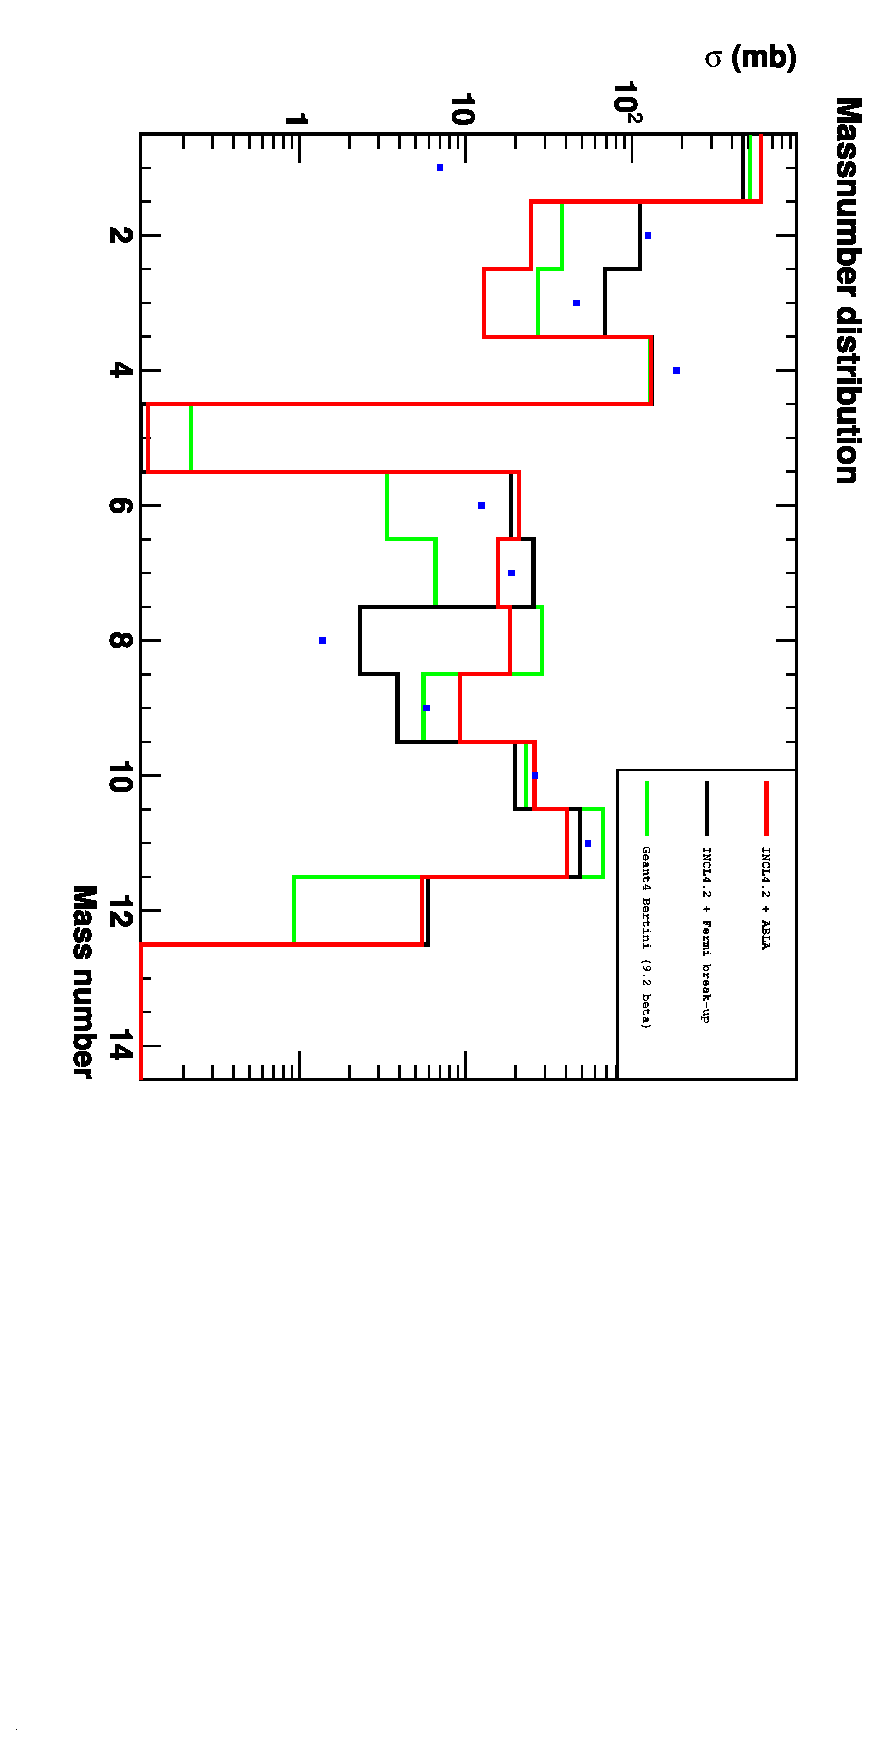
\includegraphics[scale=0.60,angle=90]{poster/images/masses.eps}
%%\end{center}
%\caption{Comparison of massnumber distributions given INCL4.2 cascade with ABLA evaporation 
%and with standard Geant4 Fermi break up model against data from \cite{a}.
%Also, results from Geant4 Bertini cascade with independent evaporation model are shown. }
%\label{fig:fermibreakup}
%\end{figure}


\begin{figure}[h]
\begin{minipage}{9.0cm}
%\begin{center}
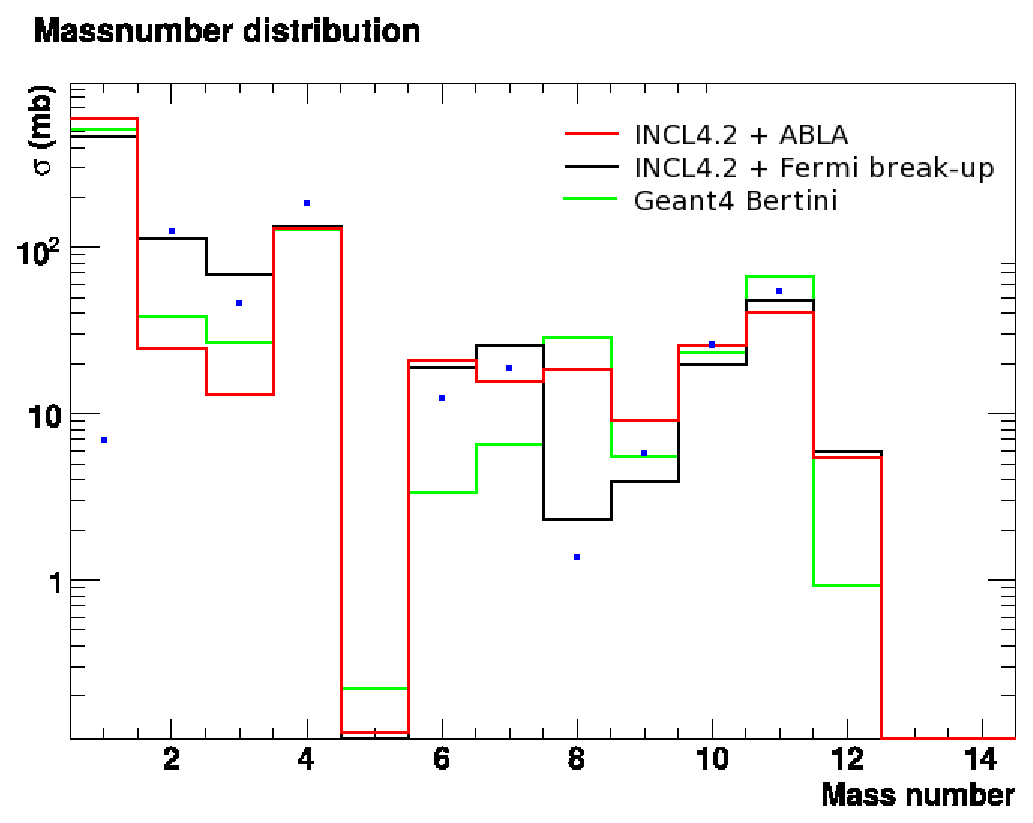
\includegraphics[width=1.0\textwidth]{poster/images/masses2.eps}
%\end{center}
%\caption{\label{label}Figure caption .}
\end{minipage}\hspace{2pc}%
\begin{minipage}{6cm}
%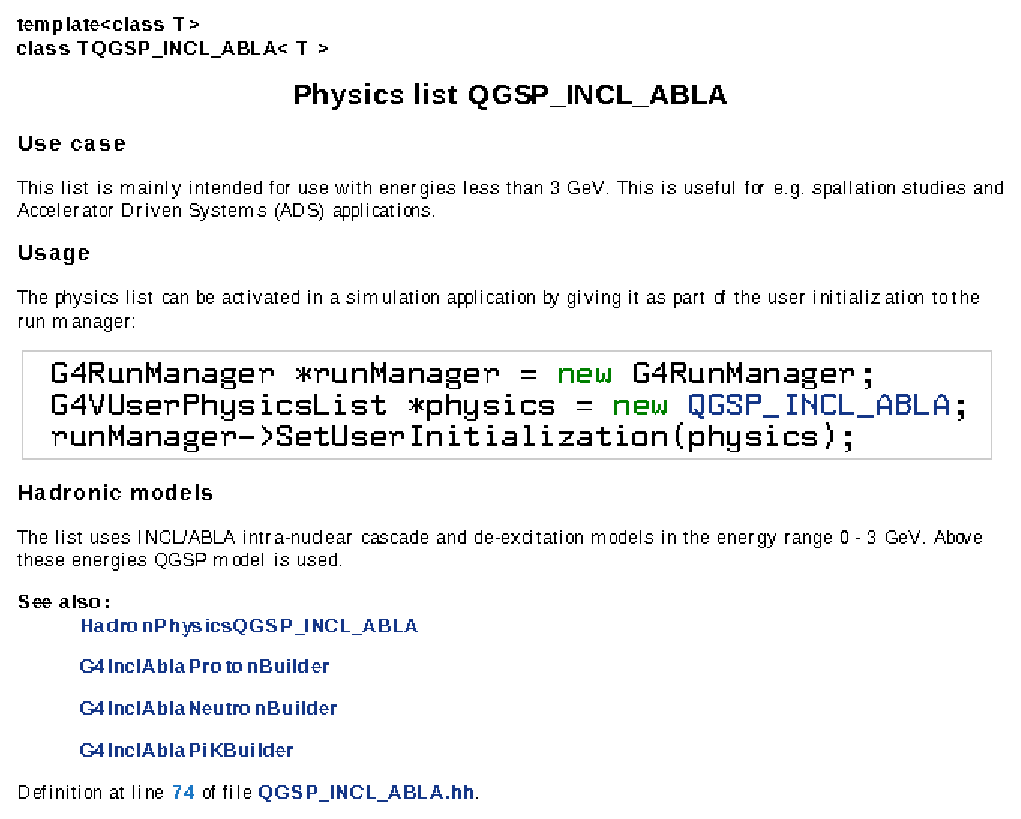
\includegraphics[width=14pc]{./poster/images/inclAblaDoc.eps}
\caption{Comparison of massnumber distributions given INCL4.2 cascade with ABLA evaporation 
and with standard Geant4 Fermi break up model against data from \cite{a}.
Also, results from Geant4 Bertini cascade with independent evaporation model are shown. }
\end{minipage} 
\end{figure}

\section{Carbon projectiles}\label{sec:carbon}

Standard INCL4.2 contains support for light ion projectiles up to and
including $\alpha$s. The INCL4.2 method of handling composite projectiles
is a simple extension of the single projectile particle case. Instead
of shooting a single projectile particle we shoot an ion that consists
of protons and neutrons.
This support is being extended to include carbon ions, 
commonly used in medical applications.
Carbon beams are of particular interest for medical applications of Geant4, 
and recently, a Carbon projectile support has been added to the INCL cascade. 

This ongoing work will  improve of the physics models for the treatment of light ion beams.



%\begin{figure}[h]
%\begin{minipage}{14pc}
%\begin{center}
%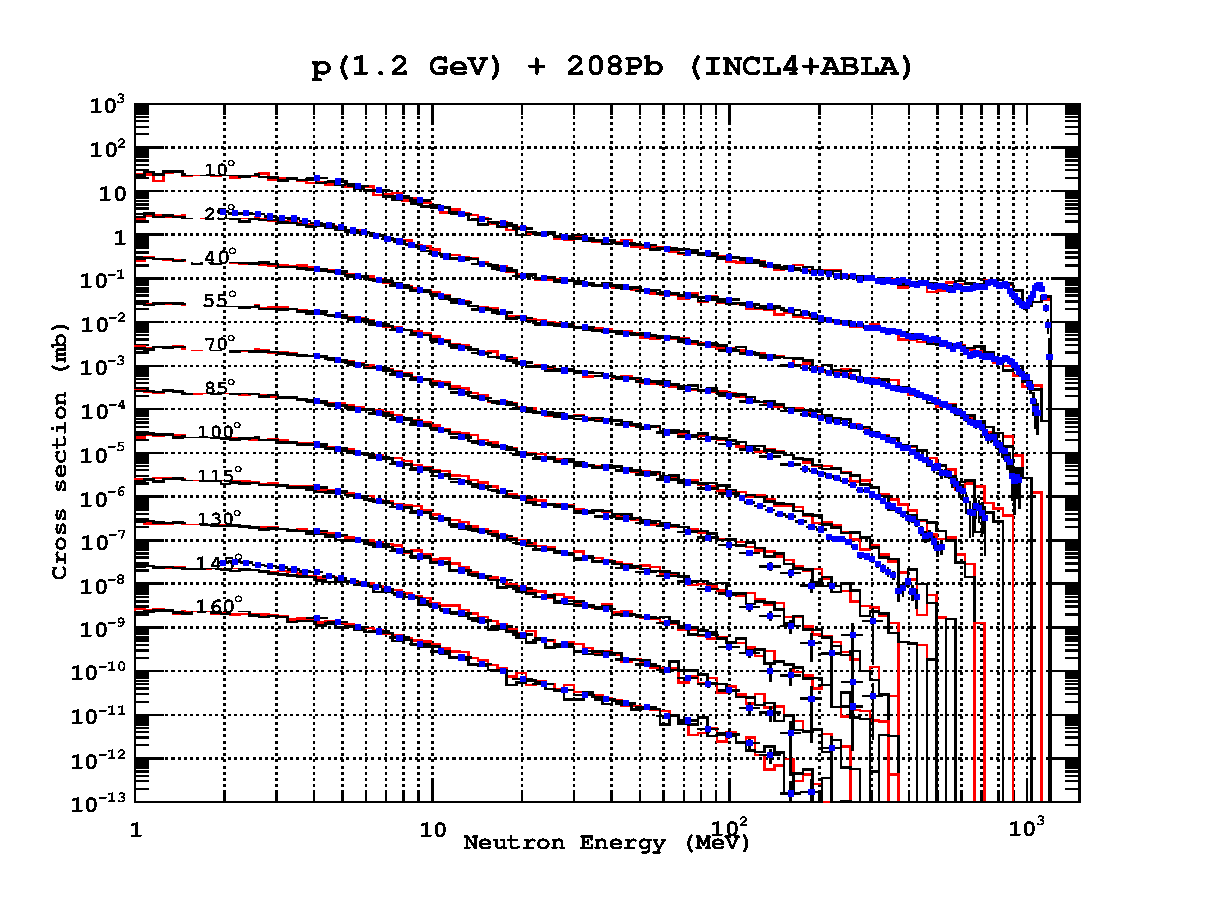
\includegraphics[width=30pc]{poster/images/lead.eps}
%\end{center}
%\caption{\label{label}Figure caption .}
%\end{minipage}\hspace{2pc}%
%\begin{minipage}{14pc}
%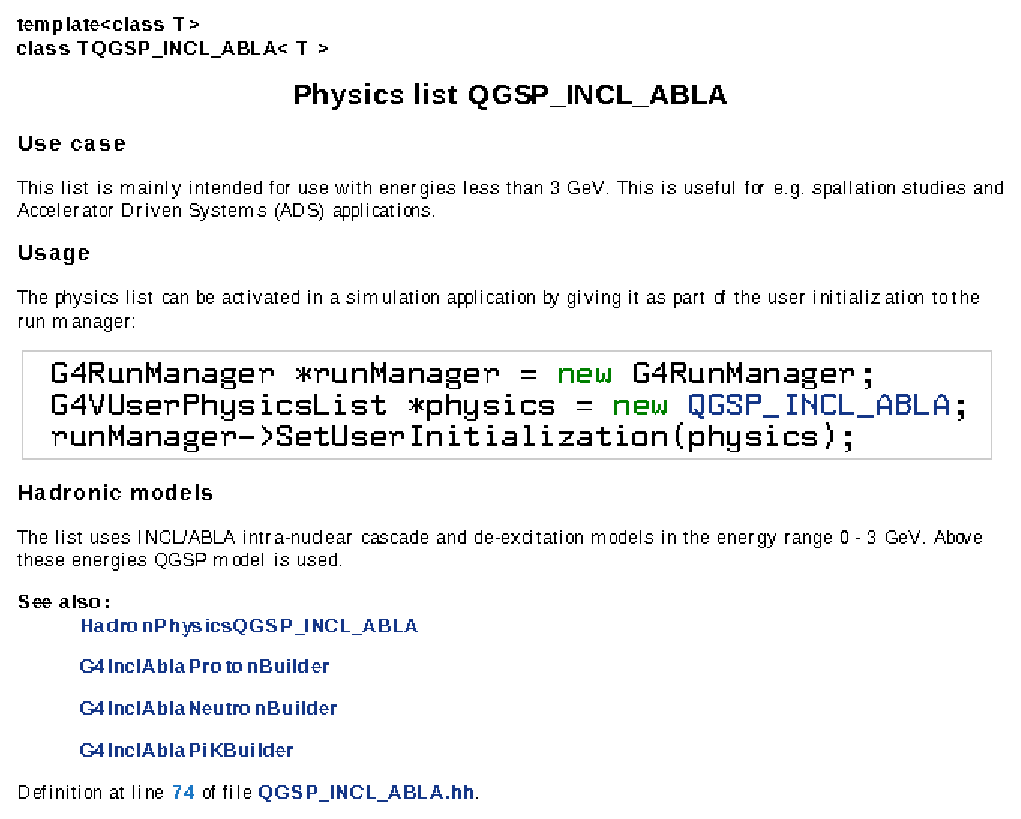
\includegraphics[width=14pc]{./poster/images/inclAblaDoc.eps}
%\caption{\label{label}Figure caption for second of two sided figures.}
%\end{minipage} 
%\end{figure}


\ack %command \ack sets the acknowledgments heading as an unnumbered section.


%\appendix % The command \appendix" is used to signify the start of the appendixes.
%\section{AH:::}

%\begin{equation}
%time= money
%\end{equation}

%To obtain a simple heading of `Appendix' use the code \verb"\section*{Appendix}". 
%If it contains numbered equations, figures or tables the command \verb"\appendix" should
%precede it and \verb"\setcounter{section}{1}" must follow it. 



\begin{center}
\begin{table}[h]
\caption{\label{opt}Summary of {\tt QGSP\_\-INCL\_ABLA} physics list~\cite{pk08bProceedings}.}
%\footnotesize\rm
\centering
\begin{tabular}{@{}*{7}{l}}
\br
Models&Description\\
\mr
\verb"Cascade model"& INCL/ABLA for protons, neutrons, $\pi^+$ and $\pi^-$\\
\verb"High energy model"& QGSP\\
\verb"Electromagnetic physics"& Geant4 standard EM\\
\br
Use-cases& \\
\br
\verb"Al-"&Targets heavier than Aluminium.\\
\verb"Particles"& proton, neutron, $\pi^+$ and $\pi^-$\\
\verb"150~MeV - 3~GeV"&Projectile energies from $\sim$ 150 MeV up to 2.5 GeV $\sim$ 3 GeV.\\
\verb"Applications"& Spallation studies, ADS \\
                   & Neutron production \\
                   & Fragment production \\
\br
\end{tabular}
\end{table}
\end{center}



\section*{References}


\begin{thebibliography}{9}

\bibitem{incl} A. Boudard et al., \emph{Intra-nuclear cascade model for
    a comprehensive description of spallation reaction data}, Phys.
  Rev. C66 (2002) 044615
\bibitem{g4} \emph{Geant4 collaboration website} \\ {\tt http://\-cern.ch/\-geant4}
\bibitem{pk08bProceedings}
A. Heikkinen, P. Kaitaniemi, and A. Boudard,
{\em Implementation of INCL4 cascade and ABLA evaporation codes in Geant4},
Journal of Physics: Conference Series 119 (2008) 032024, 
{\sf [doi:10.1088/1742-6596/119/3/032024]}
\bibitem{abla} J. Benlliure et al., \emph{Calculated nuclide
    production yields in relativistic collisions of fissile nuclei},
  Nuc. Phys. A628 (1998) 458
\bibitem{abla1} J. J. Gaimard et al., \emph{},
  Nuc. Phys. A531 (1991) 709
\bibitem{abla2} A. R. Junghans et al., \emph{},
  Nuc. Phys. A629 (1998) 635
\bibitem{gsifragments} T. Enqvist et al. \emph{},
  Nucl. Phys. A686 (2001) 481
\bibitem{g4incl} \emph{Geant4 Physics Reference Manual: INCL~4.2 Cascade and ABLA~V3 Evaporation with Fission} 
%\\ {\tt http://geant4.web.cern.ch/\-geant4/\-UserDocumentation/\-UsersGuides/\-PhysicsReferenceManual/\-html/\-node185.html}

\bibitem{data} X.Ledoux et al., \emph{Spallation Neutron Production by
  0.8, 1.2, and 1.6 GeV Protons on Pb Targets} Phys. Rev. Lett. 82
  (1999)

%\item Strite S and Morkoc H 1992 {\it J. Vac. Sci. Technol.} B {\bf 10} 1237 
\end{thebibliography}


\end{document}


